\documentclass[12t,letterpaper]{article}

\newenvironment{proof}{\noindent{\bf Proof:}}{\qed\bigskip}

\newtheorem{theorem}{Theorem}
\newtheorem{corollary}{Corollary}
\newtheorem{lemma}{Lemma} 
\newtheorem{claim}{Claim}
\newtheorem{fact}{Fact}
\newtheorem{definition}{Definition}
\newtheorem{assumption}{Assumption}
\newtheorem{observation}{Observation}
\newtheorem{example}{Example}
\newcommand{\qed}{\rule{7pt}{7pt}}

\newcommand{\assignment}[4]{
\thispagestyle{plain} 
\newpage
\setcounter{page}{1}
\noindent
\begin{center}
\framebox{ \vbox{ \hbox to 6.28in
        {\bf CS 164: Compilers\hfill #1}
\vspace{4mm}
\hbox to 6.28in
{\hspace{2.5in}\large\mbox{#2}}
\vspace{4mm}
\hbox to 6.28in
{{\it Handed Out: #3 \hfill Due: #4}}
}}
\end{center}
}

\newcommand{\solution}[3]{
\thispagestyle{plain} 
\newpage
\setcounter{page}{1}
\noindent
\begin{center}
\framebox{ \vbox{ \hbox to 6.28in
{\bf CS 164\hfill #3}
\vspace{4mm}
\hbox to 6.28in
{\hspace{2.5in}\large\mbox{#2}}
\vspace{4mm}
\hbox to 6.28in
{#1 \hfill}
}}
\end{center}
\markright{#1}
}

\newenvironment{algorithm}
{\begin{center}
\begin{tabular}{|l|}
\hline
\begin{minipage}{1in}
\begin{tabbing}
\quad\=\qquad\=\qquad\=\qquad\=\qquad\=\qquad\=\qquad\=\kill}
{\end{tabbing}
\end{minipage} \\
\hline
\end{tabular}
\end{center}}

\def\Comment#1{\textsf{\textsl{$\langle\!\langle$#1\/$\rangle\!\rangle$}}}


\usepackage{amsmath, verbatim, tikz, float}

\usetikzlibrary{arrows,automata}

\oddsidemargin 0in
\evensidemargin 0in
\textwidth 6.5in
\topmargin -0.5in
\textheight 9.0in
\newcommand{\norm}[1]{\left\lVert #1 \right\rVert}
\newcommand{\?}{\stackrel{?}{=}}

\begin{document}

\solution{Nikhil Unni (cs164-es), Section : Monday 3pm}{WA1}{Fall 2015}
\pagestyle{myheadings}


\begin{enumerate}
    \item Give a DFA for the following languages over the alphabet $\Sigma = \{a,b\}$:
    \begin{itemize}
      \item All strings that contain at most two a's.\\
        \begin{figure}[H]
        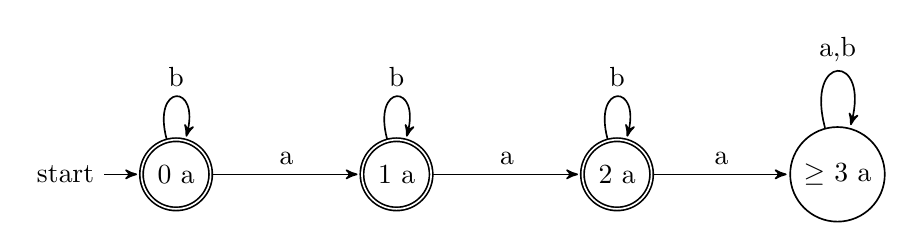
\begin{tikzpicture}[->,>=stealth',shorten >=1pt,auto,node distance=2.8cm, semithick]
          \tikzstyle{every state}=[fill=none,draw=black,text=black]
          \node[initial,state,accepting] (A)              {0 a};
          \node[state,accepting]         (B) [right of=A] {1 a};
          \node[state,accepting]         (C) [right of=B] {2 a};
          \node[state]                   (D) [right of=C] {$\geq$ 3 a};

          \path (A) edge              node {a}   (B)
                    edge [loop above] node {b}   (A)
                (B) edge              node {a}   (C)
                    edge [loop above] node {b}   (B)
                (C) edge              node {a}   (D)
                    edge [loop above] node {b}   (C)
                (D) edge [loop above] node {a,b} (D);
        \end{tikzpicture}
        \end{figure}
      \item All strings that contain at most one b.\\
        \begin{figure}[H]
        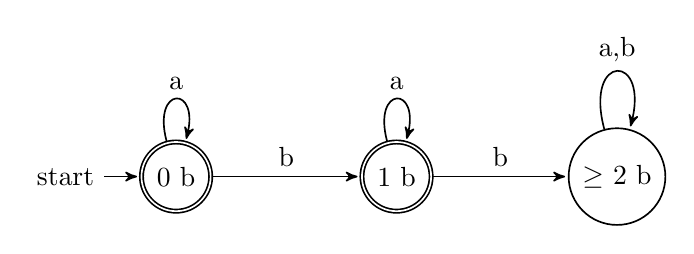
\begin{tikzpicture}[->,>=stealth',shorten >=1pt,auto,node distance=2.8cm, semithick]
          \tikzstyle{every state}=[fill=none,draw=black,text=black]
          \node[initial,state,accepting] (A)              {0 b};
          \node[state,accepting]         (B) [right of=A] {1 b};
          \node[state]                   (C) [right of=B] {$\geq$ 2 b};

          \path (A) edge              node {b}   (B)
                    edge [loop above] node {a}   (A)
                (B) edge              node {b}   (C)
                    edge [loop above] node {a}   (B)
                (C) edge [loop above] node {a,b} (C);
        \end{tikzpicture}
        \end{figure}
      \item All strings that contain at most two a's and at most one b.\\
        \begin{figure}[H]
        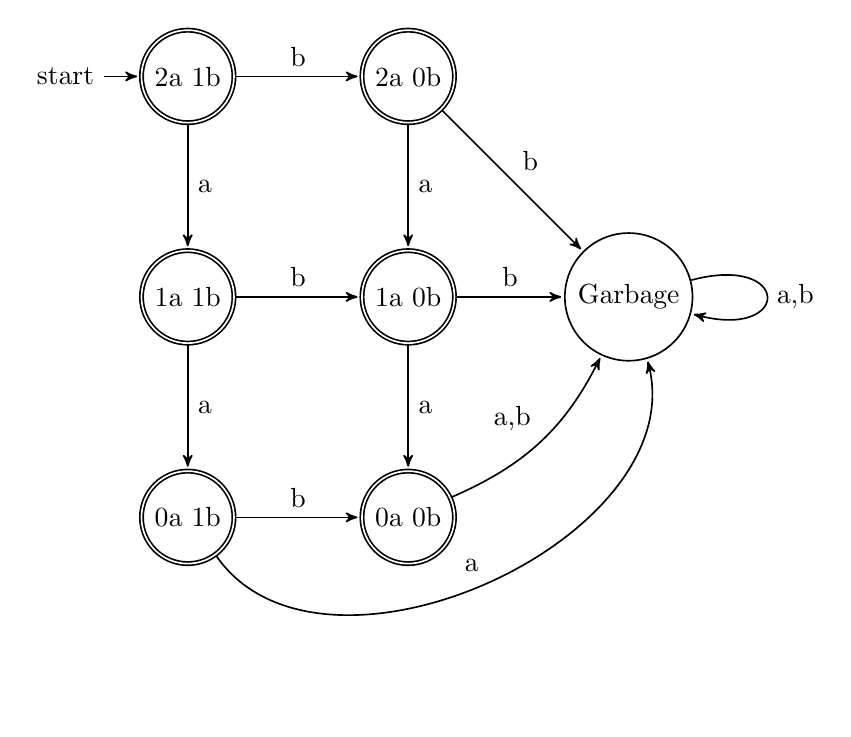
\begin{tikzpicture}[->,>=stealth',shorten >=1pt,auto,node distance=2.8cm, semithick]
          \tikzstyle{every state}=[fill=none,draw=black,text=black]
          \node[initial,state,accepting] (A)              {2a 1b};
          \node[state,accepting]         (B) [right of=A] {2a 0b};
          \node[state,accepting]         (C) [below of=A] {1a 1b};
          \node[state,accepting]         (D) [right of=C] {1a 0b};
          \node[state,accepting]         (E) [below of=C] {0a 1b};
          \node[state,accepting]         (F) [right of=E] {0a 0b};
          \node[state]                   (G) [right of=D] {Garbage};

          \path (A) edge                 node {b}   (B)
                    edge                 node {a}   (C)
                (B) edge                 node {b}   (G)
                    edge                 node {a}   (D)
                (C) edge                 node {b}   (D)
                    edge                 node {a}   (E)
                (D) edge                 node {b}   (G)
                    edge                 node {a}   (F)
                (E) edge                 node {b}   (F)
                    edge [bend right=80] node {a}   (G)
                (F) edge [bend right=20] node {a,b} (G)
                (G) edge [loop right]    node {a,b} (G);
        \end{tikzpicture}
        \end{figure}
      \item All strings that contain at least one a and no b's.\\
        \begin{figure}[H]
        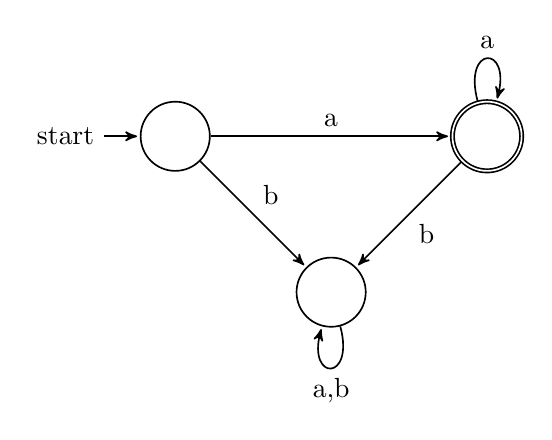
\begin{tikzpicture}[->,>=stealth',shorten >=1pt,auto,node distance=2.8cm, semithick]
          \tikzstyle{every state}=[fill=none,draw=black,text=black]
          \node[initial,state]    (A)                    {};
          \node[state]            (B) [below right of=A] {};
          \node[state,accepting]  (C) [above right of=B] {};

          \path (A) edge              node {a}   (C)
                    edge              node {b}   (B)
                (B) edge [loop below] node {a,b} (B)
                (C) edge [loop above] node {a}   (C)
                    edge              node {b}   (B);
        \end{tikzpicture}
        \end{figure}

    \end{itemize}
  \item Consider the following DFA over the alphabet $\Sigma = \{a,b\}$. (Not pictured.)\\
    Give a one sentence description of the language recognized by the DFA. Write a regular expression for the same language.\\\\

    It is the set of words where the number of a's is divisible by 4. It can be represented by the regex $b^*(ab^*ab^*ab^*ab^*)^*$.
  \item Let $\Sigma_m = \{a_1, \cdots, a_m\}$ be an alphabet containing $m$ elements, for some integer $m \geq 2$. Let $L_m$ be the following language that includes all strings in which at least one of the characters occurs an odd number of times and one of the characters occurs an even number of times.\\\\

    Construct a DFA for the language $L_2$.
        \begin{figure}[H]
        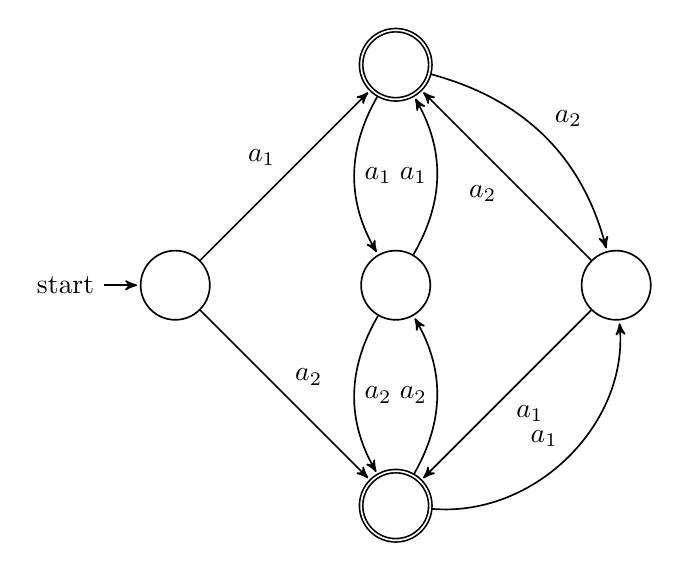
\begin{tikzpicture}[->,>=stealth',shorten >=1pt,auto,node distance=2.8cm, semithick]
          \tikzstyle{every state}=[fill=none,draw=black,text=black]
          \node[initial,state]   (A)              {};
          \node[state]           (B) [right of=A] {};
          \node[state]           (C) [right of=B] {};
          \node[state,accepting] (D) [above of=B] {};
          \node[state,accepting] (E) [below of=B] {};

          \path (A) edge node {$a_1$} (D)
                    edge node {$a_2$} (E)
                (B) edge [bend right=30] node {$a_1$} (D)
                    edge [bend right=30] node {$a_2$} (E)
                (C) edge node {$a_2$} (D)
                    edge node {$a_1$} (E)
                (D) edge [bend right=30] node {$a_1$} (B)
                    edge [bend left=30] node {$a_2$} (C)
                (E) edge [bend right=30] node {$a_2$} (B)
                    edge [bend right=50] node {$a_1$} (C);

        \end{tikzpicture}
        \end{figure}
    Also construct an NFA for the language $L_3$.    
        \begin{figure}[H]
        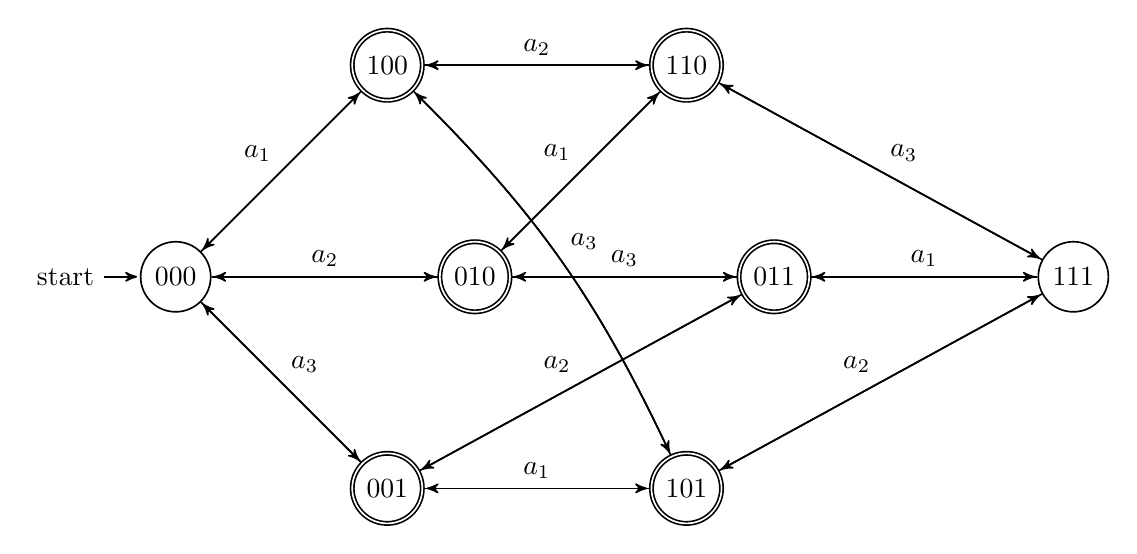
\begin{tikzpicture}[->,>=stealth',shorten >=1pt,auto,node distance=3.8cm, semithick]
          \tikzstyle{every state}=[fill=none,draw=black,text=black]
          \node[initial,state]   (A)                    {000};
          \node[state,accepting] (B) [above right of=A] {100};
          \node[state,accepting] (C) [right of=A]       {010};
          \node[state,accepting] (D) [below right of=A] {001};
          \node[state,accepting] (E) [right of=B]       {110};
          \node[state,accepting] (F) [right of=D]       {101};
          \node[state,accepting] (G) [right of=C]       {011};
          \node[state]           (H) [right of=G]       {111};

          \path (A) edge node {$a_1$} (B)
                    edge node {$a_2$} (C)
                    edge node {$a_3$} (D)
                (B) edge node {} (A)
                    edge node {$a_2$} (E)
                    edge [bend left=10] node {$a_3$} (F)
                (C) edge node {$a_1$} (E)
                    edge node {} (A)
                    edge node {$a_3$} (G)
                (D) edge node {$a_1$} (F)
                    edge node {$a_2$} (G)
                    edge node {} (A)
                (E) edge node {} (C)
                    edge node {} (B)
                    edge node {$a_3$} (H)
                (F) edge node {} (D)
                    edge node {$a_2$} (H)
                    edge [bend right=10] node {} (B)
                (G) edge node {$a_1$} (H)
                    edge node {} (D)
                    edge node {} (C)
                (H) edge node {} (E)
                    edge node {} (F)
                    edge node {} (G);
        \end{tikzpicture}
        \end{figure}
        In the diagram, the nodes are labeled ``001'' or ``011'' for instance. This just means that, at index $i$, if it is a 0, that means the number of $a_{i+1}$ is even, or its odd if the character is 1. Also, another note -- I drew double arrows for the transitions, which officially means : if there's a double arrow with character $a$ between two nodes $q_0$ and $q_1$, you can transition from $q_0$ to $q_1$ with $a$, and you can transition from $q_1$ to $q_0$ with $a$. I only did it this way because without the double arrows, an already hard to read graph became an impossible to read graph.

        \item 
        \begin{enumerate}
          \item Determine whether or not the following languages are regular. Explain why in one or two sentences.
            \begin{itemize}
              \item $L_1$: All strings over the alphabet $\{0,1\}$ that have a different number of 1's and 0's.\\\\
                Not regular, because there's no \textbf{finite} ``mechanism'' for keeping track of the differences in 0's and 1's that we've seen so far.\\
              \item $L_2$: All strings over the alphabet $\{0,1\}$ that are not repeating sequences.\\\\
                Not regular, because there's no way to ``remember'' the (arbitrary amount of) nodes we've seen before. It can by shown by the Pumping Lemma that since the sequence we have to remember can be of arbitrarily long length, there's no way that there can be a DFA that accepts the language.\\

              \item $L_3$: All words that have ever existed and will ever exist in the English language (Assume there is a maximum word ength since humans have limited breath).\\\\
                Because there is a maximum word length, call it $n$ characters long, the total number of words is a finite $26^{n}$ (or some number greater than 26 if humans develop new characters... but certainly a finite alphabet length). And since all finite languages are regular (we can construct a DFA/Trie for the set of all possible words), $L_3$ is regular.
            \end{itemize}
        \end{enumerate}
\end{enumerate}

\end{document}
